\documentclass[crop,dvisvgm,border=4pt]{standalone}

\usepackage{amsmath,amssymb}
  \usepackage{CJKutf8}
  \newcommand{\llbracket}{[\![}
  \newcommand{\rrbracket}{]\!]}
  \usepackage{tikz-cd}
  \usetikzlibrary{arrows.meta,backgrounds,calc,decorations.pathreplacing,fit,positioning,shapes.geometric}
  \newcommand{\pbcorner}{\vcenter{\hbox{\tikz[scale=.22]{\draw[line width=.55pt] (0,1)--(0,0)--(1,0);}}}}

\begin{document}
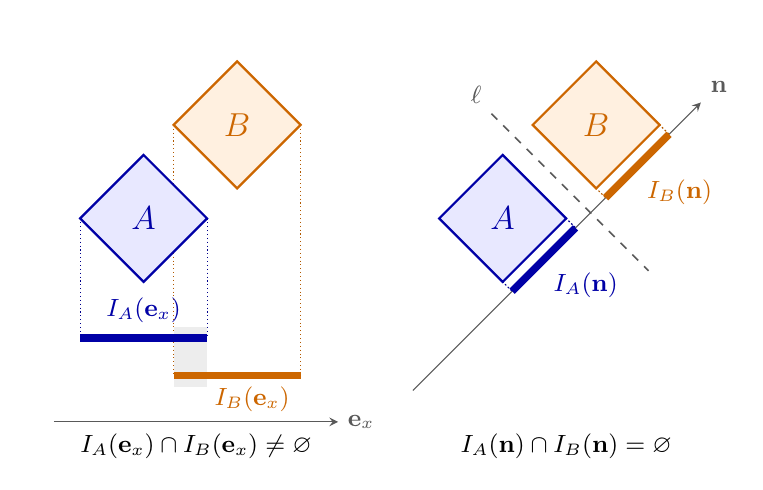
\begin{tikzpicture}[
  x=.95cm,y=.95cm,>=stealth,font=\small,
  boxA/.style={draw=blue!65!black,fill=blue!9,thick},
  boxB/.style={draw=orange!80!black,fill=orange!12,thick},
  projectA/.style={blue!55!black,densely dotted,thin},
  projectB/.style={orange!70!black,densely dotted,thin}
]
\path[use as bounding box] (-.35,-1.15) rectangle (9.1,4.65);
\pgfmathsetmacro{\satradius}{.6*sqrt(2)}
\pgfmathsetmacro{\sathalfprojection}{.6/sqrt(2)}
\foreach \panel in {0,1} {
  \begin{scope}[shift={({4.8*\panel},0)}]
    \coordinate (AL) at ({1.2-\satradius},2.1);
    \coordinate (AT) at (1.2,{2.1+\satradius});
    \coordinate (AR) at ({1.2+\satradius},2.1);
    \coordinate (AB) at (1.2,{2.1-\satradius});
    \coordinate (BL) at ({2.45-\satradius},3.35);
    \coordinate (BT) at (2.45,{3.35+\satradius});
    \coordinate (BR) at ({2.45+\satradius},3.35);
    \coordinate (BB) at (2.45,{3.35-\satradius});
    \ifnum\panel=0
      \fill[black!7] ({2.45-\satradius},-.15) rectangle ({1.2+\satradius},.65);
      \coordinate (AP0) at ({1.2-\satradius},.5);
      \coordinate (AP1) at ({1.2+\satradius},.5);
      \coordinate (BP0) at ({2.45-\satradius},0);
      \coordinate (BP1) at ({2.45+\satradius},0);
      \draw[projectA] (AL) -- (AP0) (AR) -- (AP1);
      \draw[projectB] (BL) -- (BP0) (BR) -- (BP1);
      \draw[->,black!65] (0,-.62) -- (3.8,-.62) node[right] {$\mathbf e_x$};
      \draw[blue!65!black,line width=2.7pt] (AP0) -- (AP1);
      \draw[orange!80!black,line width=2.7pt] (BP0) -- (BP1);
      \node[blue!65!black,above] at (1.2,.57) {$I_A(\mathbf e_x)$};
      \node[orange!80!black,below] at (2.65,-.02) {$I_B(\mathbf e_x)$};
      \node at (1.9,-.95) {$I_A(\mathbf e_x)\cap I_B(\mathbf e_x)\ne\varnothing$};
    \else
      \coordinate (AP0) at ({1.75-\sathalfprojection},{1.55-\sathalfprojection});
      \coordinate (AP1) at ({1.75+\sathalfprojection},{1.55+\sathalfprojection});
      \coordinate (BP0) at ({3-\sathalfprojection},{2.8-\sathalfprojection});
      \coordinate (BP1) at ({3+\sathalfprojection},{2.8+\sathalfprojection});
      \draw[projectA] (AL) -- (AP0) (AB) -- (AP0) (AT) -- (AP1) (AR) -- (AP1);
      \draw[projectB] (BL) -- (BP0) (BB) -- (BP0) (BT) -- (BP1) (BR) -- (BP1);
      \draw[->,black!65] (0,-.2) -- (3.85,3.65) node[above right] {$\mathbf n$};
      \draw[blue!65!black,line width=2.7pt] (AP0) -- (AP1);
      \draw[orange!80!black,line width=2.7pt] (BP0) -- (BP1);
      \node[blue!65!black,below right] at (1.75,1.5) {$I_A(\mathbf n)$};
      \node[orange!80!black,below right] at (3,2.75) {$I_B(\mathbf n)$};
      \draw[black!65,dashed,semithick] (1.05,3.5) node[above left] {$\ell$} -- (3.15,1.4);
      \node at (2.05,-.95) {$I_A(\mathbf n)\cap I_B(\mathbf n)=\varnothing$};
    \fi
    \path[boxA] (AL) -- (AT) -- (AR) -- (AB) -- cycle;
    \path[boxB] (BL) -- (BT) -- (BR) -- (BB) -- cycle;
    \node[blue!65!black,font=\large] at (1.2,2.1) {$A$};
    \node[orange!80!black,font=\large] at (2.45,3.35) {$B$};
  \end{scope}
}
\end{tikzpicture}
\end{document}
